\documentclass{article}
\usepackage[utf8]{inputenc}
\usepackage[greek, brazil]{babel}
\usepackage[left=1cm, right=1.5cm, top=1.5cm, bottom=1.5cm]{geometry}
\usepackage{hyperref}
\usepackage[usenames,dvipsnames]{xcolor}
\usepackage{graphics}

\hypersetup {
  colorlinks,
  citecolor = NavyBlue,
  filecolor = NavyBlue,
  linkcolor = NavyBlue,
  urlcolor = NavyBlue
}

\author {
  Lucas Skywalker
}
\title {
  Dynamic Linked Library (.dll) e Shared Object (.so)\\
  {
    \small estudo
  }
}
\date{\today}

\begin{document}

\maketitle

\section{Intro}
As .dll ou .so são bibliotecas que contém rotinas já previamente compiladas.
Para que o processo de reutilização dessas rotinas pelo seus programas seja mais
ágil e menos custoso, pois se prevê que serão reutilizadas muitas vezes pelos
seus programas.

\section{Estabelecendo ligação dinâmica pela primeira vez}

  \begin{enumerate}
    \item De repente o sistema operacional se depara com uma rotina não local,
    ele gera um desvio para poder resolver o problema que apareceu para ele, de
    uma rotina contida em algum .dll ou .so, que será um \verb|jal [LABEL1]| (o
    jal é porque ele deve retornar ao PC+4 depois dessa chamada para rotinas.)

    \item A [LABEL1] é o local dentro do programa que irá ler a memória onde
    está guardada o endereço da sua rotina não local, isto é, ele irá executar
    lw \$s1, [LABEL2], corregando o endereço da rotina não local em um
    registrador (neste caso \$s1), e logo após irá executar um jr \$s1 para
    desviar para o valor contido no endereço [LABEL2]. Como é a nossa primeira
    execução, o valor dentro de [LABEL2] não é a rotina que nós queremos ainda,
    ao invés disso ele irá ter o endereço do identificador da rotina, logo ele
    irá desviar para o identificador.

    \item O código do identificador da rotina não local que o programa quer,
    será visto pelo montador como um \verb|li $s0, I| (li = load immediate),
    logo após carregar \textbf{[LC]} ele desviará para o ligador/carregador
    (LC).

    \item O LC irá caregar o código da rotina em memória e irá mapear o endereço
    do código para o endereço da memória [LABEL2], aí então ele desviará para a
    torina não local e a rotina será executada.

    \item Executa a rotina não local e retorna para o programa.
  \end{enumerate}

  \pagebreak
  \begin{figure}
    \centering
    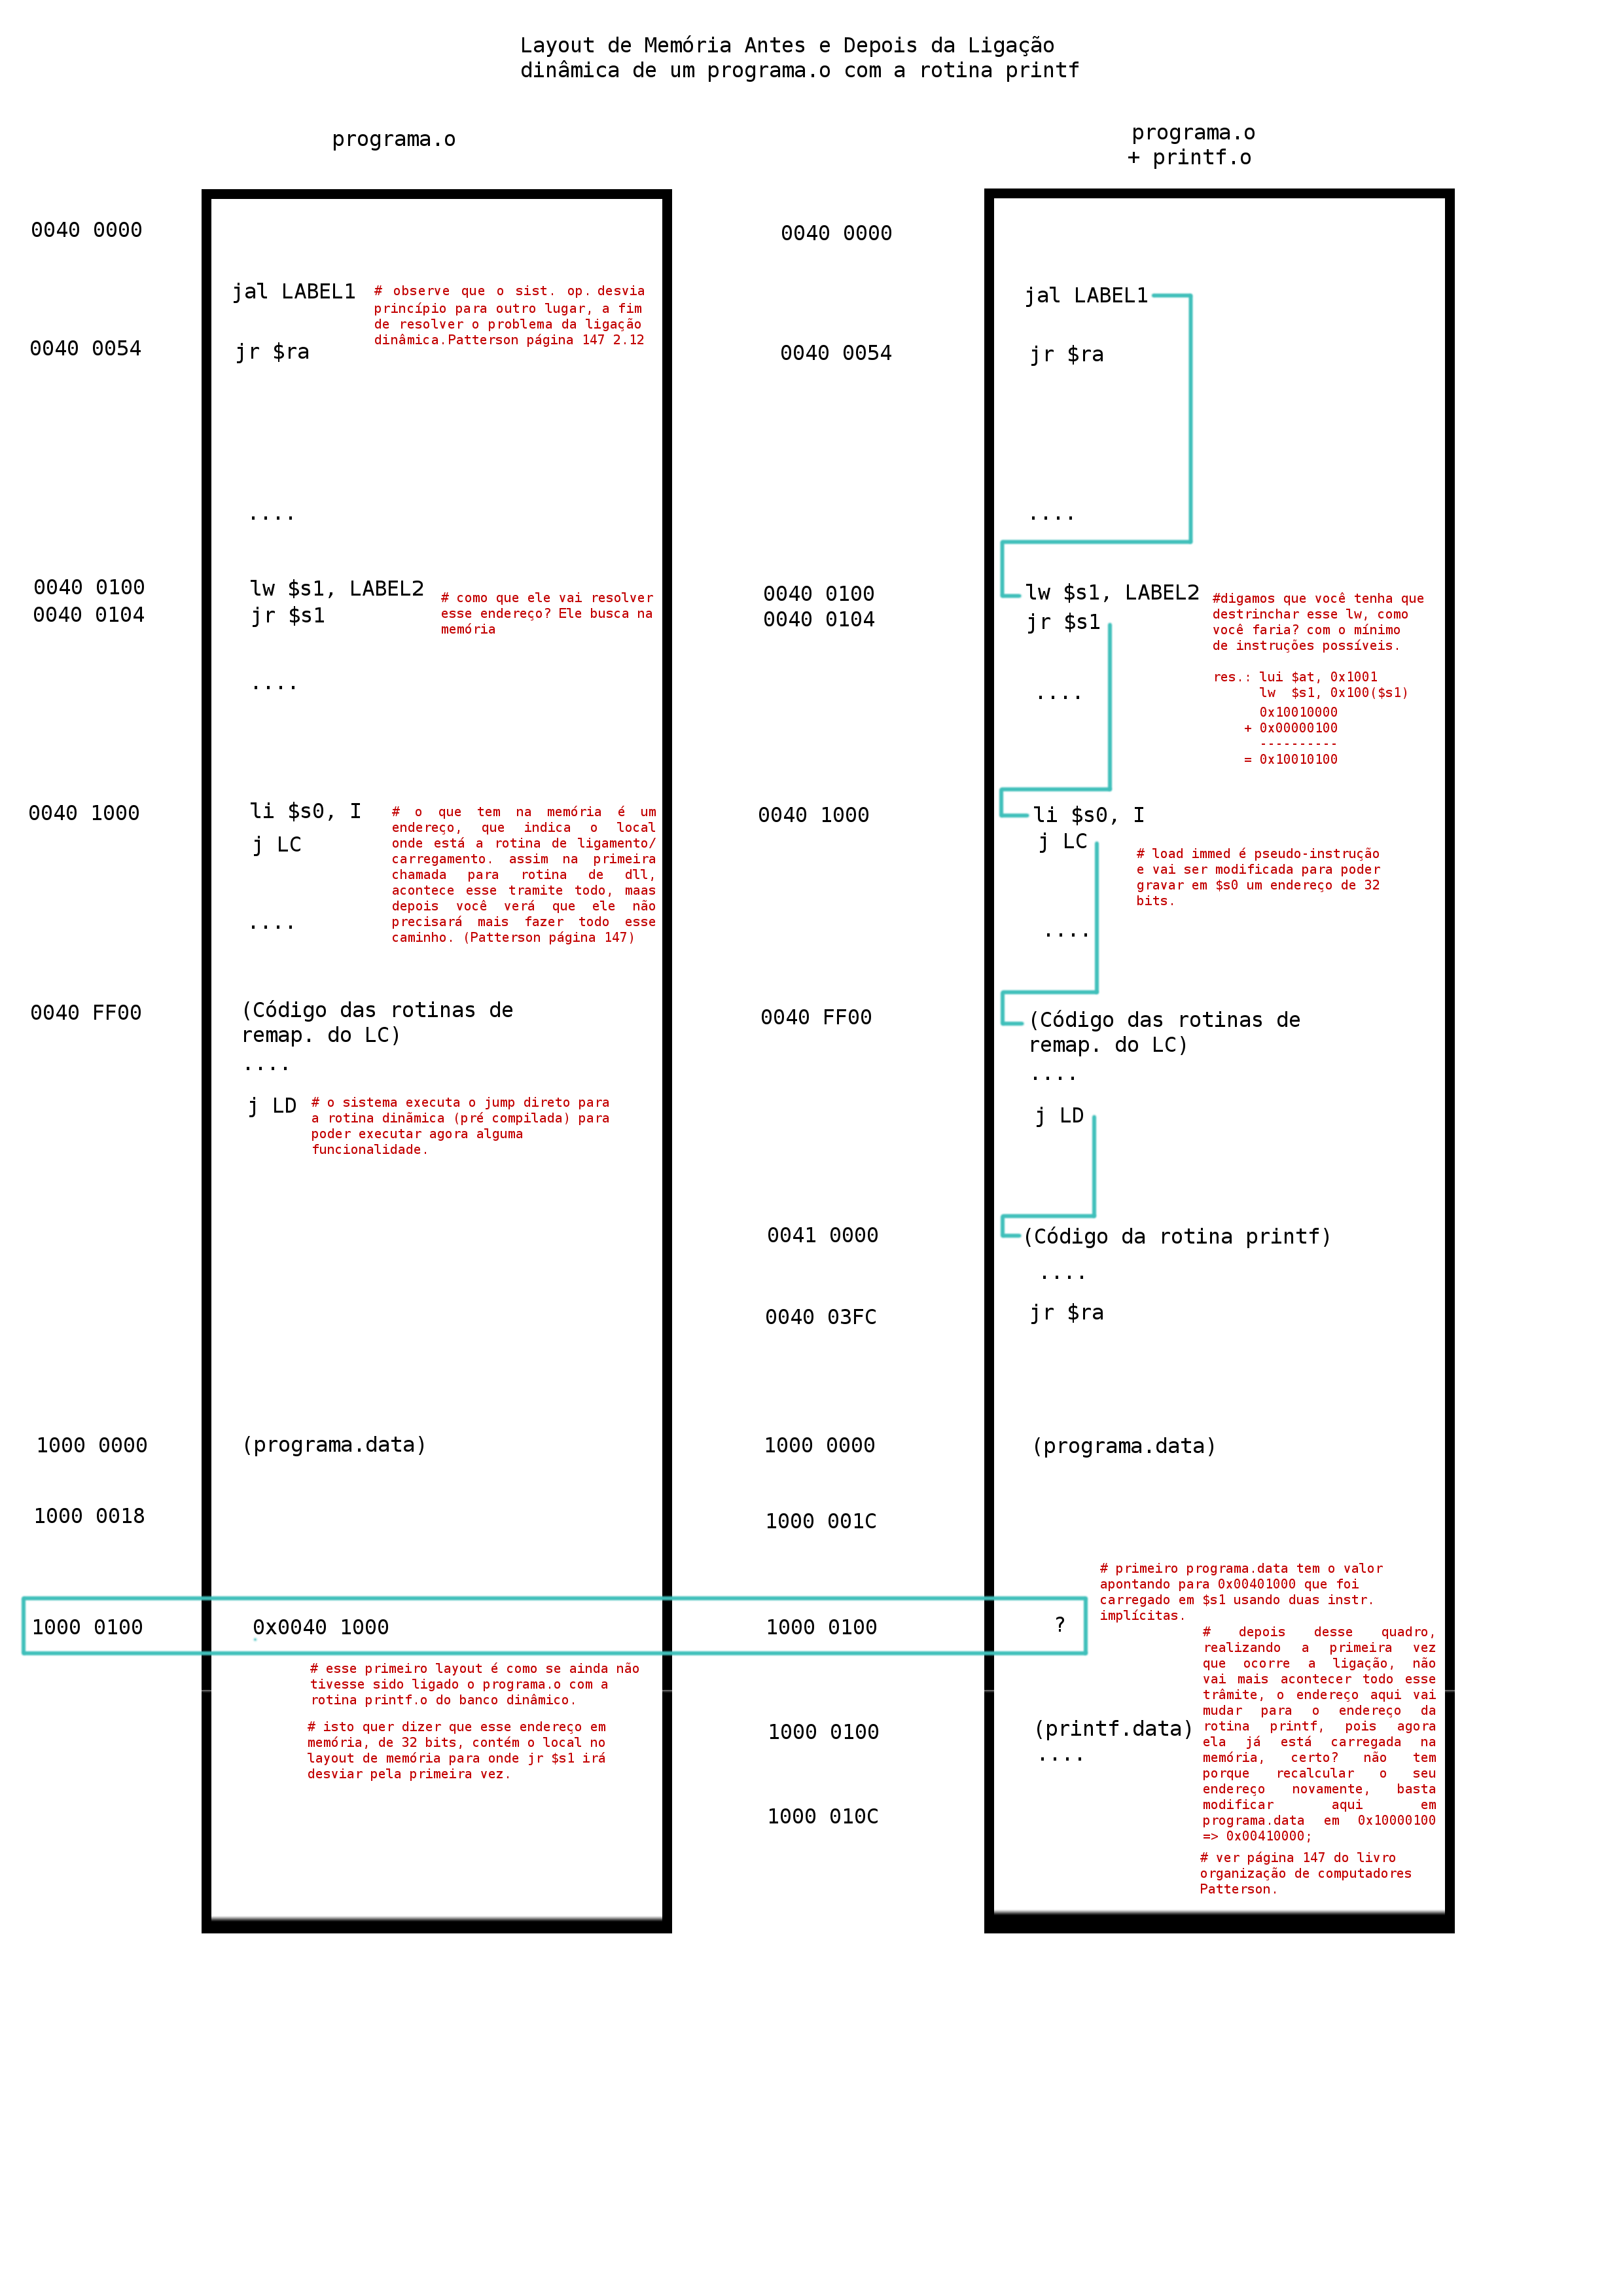
\includegraphics{dll-so.png}
  \end{figure}

\end{document}
